\section{Background and Motivation}
\label{sec:background}

% 中文导读（仅供写作与审阅，不进入最终 PDF）：
% 本节按照“故障恢复为什么变贵 -> 为什么不同请求的恢复价值不同 -> 为什么现有 KV 管理缺少必要信息”展开。
% 1. agentic workflow -> retry 需要重算的前缀通常越长，因此长上下文放大恢复代价。
% 2. Workflow Completion Time（WCT）， Slack。
% 3. 现有推理引擎主要依据 KV 大小、位置、复用和系统负载管理缓存，却缺少 workflow 依赖与 Slack；
% 因此 KV Priority 应由上层 agentic 信息决定，并表示为一个 chunk 对 failure-induced WCT 的边际降低。

% 本节主文只保留一组 Motivation 图像：
% Figure~\ref{fig:real-cc-parallel}：三个子图使用同一 Real CC trace；依次给出严格并行
%    subagent 秒差 CDF、可编辑 Draw.io workflow 实例、以及 failure-position counterfactual。
% figures/motivation-recovery-scaling.pdf 与
% figures/motivation-kv-publication-comparison.pdf 移入 appendix/implementation audit；
% 未校准 component model 不占用主文 Motivation 空间。

\subsection{Agentic context growth amplifies GPU-failure recovery cost}

An agentic application is a DAG of model and tool calls whose later requests
consume an accumulated transcript.  Prefix caching can reuse prior KV, but
each tool return still starts a new admission/prefill/decode lifecycle
~\cite{abhyankar2024infercept}.  Context and KV therefore tend to grow across
turns.  A worker failure discards this execution state; a compatible prefix can
avoid re-prefill, while an absent suffix must be recomputed.

Already generated KV is immutable under a fixed model and token sequence, so
the runtime seals it in groups of $G$ tokens.  Only a complete contiguous
prefix is a recovery point.  Decisions are online: future groups and final
length are unknown; per-request checkpoints are coarse, whereas independent
chunk rewards double-count overlapping prefixes.  \system{} instead values
prefix-bundle actions whose recovery plan may combine peer HBM, Store reads,
and recomputation.  Service bounds include setup, contention, adoption, and
resume rather than hardware peak bandwidth.  Protection consumes HBM, Store
quota, and transfer capacity also needed by healthy traffic, so the objective
must price workflow benefit without imposing a normal-path tax.  Evaluation
separates component bounds from physical failure-to-ready time.

\subsection{Workflow completion exposes critical requests}

The user-visible unit is workflow completion time
$\mathrm{WCT}_w=C_w-A_w$.  We measure fault-added
$[\mathrm{WCT}^{\mathrm{fail}}_w-\mathrm{WCT}^{\mathrm{nf}}_w]_+$ against a
paired no-failure run, so changing the healthy schedule cannot masquerade as
recovery benefit.  A request matters only through delay propagated to the
terminal: one branch can block a fan-in while another absorbs the same pause.

Figure~\ref{fig:real-cc-parallel} quantifies this structure in the public Real
CC trace~\cite{semianalysis2026cctraces}.  A parser fan-out is a maximal
consecutive run of top-level subagent records with at least two branches; we
retain it only when all recorded branch intervals share a nonempty common
overlap.  For fan-out $g$, let
$R_g=\max_{a\in g}d_a-\min_{a\in g}d_a$.  Each workflow contributes one CDF
sample, $R_w=\max_{g\in G_w}R_g$, so workflows with many fan-outs are not
overweighted and branches from different episodes are never compared.  Of 393
workflows, 124 contain 292 retained fan-outs and 944 branch executions.  The
median $R_w$ is 140.611~s and the 90th percentile is 1570.290~s.

Panels~(b,c) use workflow 8ab0a089\ldots: five branches last 110.3, 116.7,
78.9, 117.9, and 107.1~s (39.0~s gap).  Because the trace has no parent ID, we
reconstruct its isolated fan-out/fan-in from top-level order and timestamps.
At common active time $t_f=349.5$~s, panel~(c) combines each real 65--112K
prefix and observed fan-in slack with the Qwen3-235B-A22B
TP8$\times$PP4$\times$EP8 AIConfigurator recomputation model.  Exposed delays
are 0, 17.2, 0, 35.9, and 21.4~s.  This trace-plus-model counterfactual is not a
Claude measurement or paired failure run.

\begin{figure*}[t]
  \centering
  \begin{minipage}[b]{0.285\textwidth}
    \centering
    \parbox[c][1.72in][c]{\linewidth}{\centering
      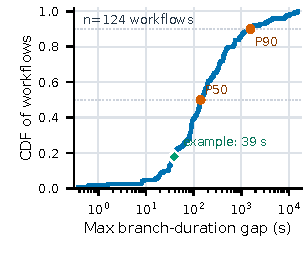
\includegraphics[width=\linewidth]{figures/real-cc-parallel-subagent-duration.pdf}}
    \small (a) Parallel-runtime gap.
  \end{minipage}\hfill
  \begin{minipage}[b]{0.39\textwidth}
    \centering
    \parbox[c][1.72in][c]{\linewidth}{\centering
      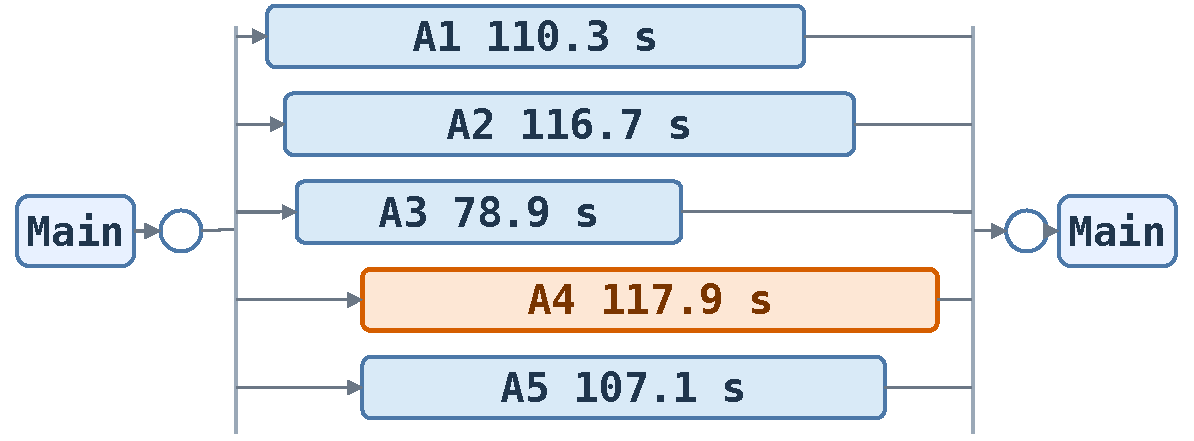
\includegraphics[width=\linewidth]{figures/real-cc-workflow-8ab0a089.pdf}}
    \small (b) Real CC workflow example.
  \end{minipage}\hfill
  \begin{minipage}[b]{0.285\textwidth}
    \centering
    \parbox[c][1.72in][c]{\linewidth}{\centering
      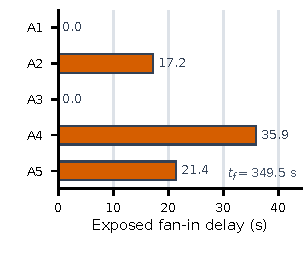
\includegraphics[width=\linewidth]{figures/real-cc-failure-position-counterfactual.pdf}}
    \small (c) Failure-position sensitivity.
  \end{minipage}
  \caption{Parallel execution and failure-position sensitivity in the Real CC
  trace.  Panel~(a) reports the CDF of each eligible workflow's largest
  within-fan-out slowest-minus-fastest duration gap.  Panel~(b) reconstructs a
  selected five-way fan-out from workflow 8ab0a089\ldots, whose
  slowest--fastest gap is 39.0~s.  Panel~(c) marks all five failure targets and
  subtracts each branch's observed fan-in slack from its configuration-predicted
  prefix-recomputation time at $t_f=349.5$~s.  Panels~(a) and~(b) summarize trace
  observations; panel~(c) is a trace-plus-AIConfigurator counterfactual rather
  than an end-to-end measurement.}
  \Description{Three panels show a Real CC workflow-level duration-gap CDF, a
  compact five-way fan-out with a 39-second branch-duration gap, and a
  horizontal-bar counterfactual for all five failure targets.}
  \label{fig:real-cc-parallel}
\end{figure*}

At each LLM-request or tool-call completion, Algorithm~1 uses a GBDT model to
predict the remaining duration $\widehat T_r(t)$ of each active branch and CPM
to identify its next mandatory fan-in.  The unknown suffix shared after that
join cancels from the comparison, so the application need not predict the
entire future workflow.  For branch $r$, it computes
\begin{equation}
  s_r(t)=\left[\max_{j\ne r}\widehat T_j(t)-\widehat T_r(t)\right]_+.
  \label{eq:slack}
\end{equation}
The next request carries this Slack as ordinary metadata.  The serving layer
decreases it by elapsed request time, and the next application response
replaces it with a new GBDT/CPM estimate.  Slack is therefore dynamic rather
than an agent label or operator SLO.  Prediction error may change protection
priority, but it cannot bypass physical resource limits or make an incomplete
KV group recoverable.

\subsection{KV priority must incorporate agentic information}

Local size, tier, recency, reuse, and load signals cannot reveal whether a
pause blocks a workflow join.  The missing input is the marginal reduction in
failure-induced WCT produced by a complete KV action, after Slack and
tier-specific resource cost.  Agentic information augments rather than replaces
the engine's placement signals.

\paragraph{Serving and workflow substrates.}
PagedAttention and SGLang provide efficient page/prefix management
~\cite{kwon2023vllm,zheng2024sglang}; Mooncake, HiCache, SYMPHONY, Strata, and
Bidaw provide disaggregated or hierarchical KV placement and loading
~\cite{qin2025mooncake,xie2025hicache,agarwal2026symphony,
xie2026strata,hu2026bidaw}.  Parrot, KVFlow, Pythia, and Agentix expose
workflow structure or predictability to serving
~\cite{lin2024parrot,pan2025kvflow,yu2026pythia,luo2026agentix}.
These are substrates, not limitations: \system{} claims neither tiering nor
DAG analysis.  Their cache state, reuse, and load signals do not alone encode
how a worker-failure pause propagates to workflow completion.

\paragraph{Agent-aware and physical KV scheduling.}
TokenCake, Continuum, PBKV, and TokenDance already use graph criticality,
waiting time, future invocation, or synchronized rounds for normal-time KV
management~\cite{bian2026tokencake,li2026continuum,
zheng2026pbkv,bian2026tokendance}.  CacheFlow overlaps recomputation and I/O
across tokens, layers, and GPUs and schedules batch restoration
~\cite{nian2026cacheflow}.  We therefore claim neither the first agent-aware
KV manager nor hybrid/parallel restoration.  A CacheFlow-like engine can
implement the restore/load/recompute path; our distinct input is workflow
Slack used both before and after a worker failure.

Configured MooncakeStoreConnector and HiCache paths may expose only a committed
prefix at a decode-time failure; the live tail still requires recomputation.
Their exact publication point depends on connector and write policy, so the
configuration-specific timeline is deferred to the appendix.  Cache presence
alone is not a crash-consistent resume contract.

\paragraph{Recovery and workflow Slack.}
D\'ej\`aVu streams KV for recovery; GhostServe, RaidServe, KevlarFlow, LUMEN,
and Concordia provide shadow/checkpoint, routing, or execution-state recovery
mechanisms~\cite{strati2024dejavu,jayakody2026ghostserve,xu2026raidserve,
qian2026kevlarflow,cao2026lumen,gan2026concordia}.  MFS schedules normal
multi-stage flows by laxity and TENT supplies deadline-aware resilient data
movement~\cite{sun2026mfs,ren2026tent}.  Thus checkpointing, load-aware
recovery, deadline fields, and flow scheduling are not our novelty.  Our
narrow claim is the coupling: the same workflow Slack values Store/peer
protection before a worker fail-stop and orders the joint
restore/load/recompute path afterward under serving-resource limits.

Classic real-time systems already use task slack to place checkpoints and
reserve rollback work, including distributed DAG tasks scheduled by EDF
~\cite{melhem2004interplay,acharya2008dynamic}.  Hence neither ``slack-aware
checkpointing'' nor Slack-ordered recovery is our novelty.  Our narrower claim
is its KV realization: compute Slack from an evolving agent workflow, use it to
value Store or peer-HBM state before fail-stop, and reuse it to order recovery
afterward.

% The archived preliminary SGLSim figure is intentionally excluded: it does
% not implement the final policy or physical recovery path.  Paper claims will
% use the final paired evaluation rather than promote that diagnostic.

\subsection{Design requirements and scope}

The design must therefore optimize workflow-visible delay over complete KV
groups, admit only failure-valid shards, isolate healthy traffic, and keep
analytical, protocol, and empirical evidence distinct.

We consider one declared fail-stop serving domain at a time and label
process/GPU and host failures separately; colocated state is lost.  The Router,
failure-isolated request log, Store quorum, network, and a model-loaded
same-layout target survive.  The Router---not \textsc{SlackLandlord}---selects that target,
which resumes from a surviving continuous prefix or recomputes.  We do not
splice pipeline stages.  Correlated/Store/Router failures, corrupted weights,
Byzantine faults, and cross-layout recovery are outside the first claim.
